\documentclass{standalone}
\usepackage[utf8]{inputenc}
\usepackage[T1]{fontenc}
\usepackage{pgfplots}
\pgfplotsset{compat=1.8}

\newcommand{\norma}[1]{\Vert #1 \Vert}

\begin{document}
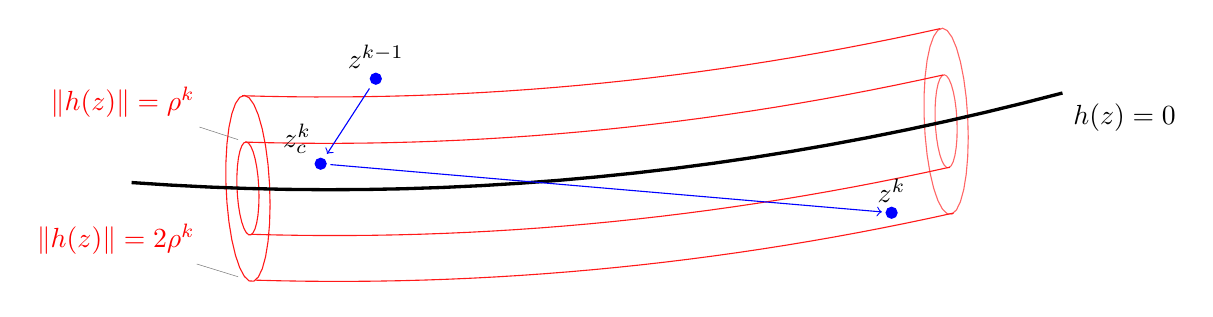
\begin{tikzpicture}
  \begin{axis}[view={70}{20}, xmin=-4.4, xmax=3.4, zmin=-1, ymax=-1.8, ymax=1.8,
      axis lines=none,
      xtick=\empty, ytick=\empty, ztick=\empty, x post scale=2.0,
      y post scale=2.5, z post scale=1.1, lightgray
    ]

    \addplot3 [domain=0:360, draw=red!90!white,
      samples=30, samples y=0]
        ({0.3*cos(x)}, {-1.2}, {0.1*1.2*1.2 + 0.3*sin(x)})
        node[pos=0.25, pin=160 : {\color{red}$\norma{h(z)}=\rho^k$}] {};
    \addplot3 [domain=0:360, draw=red!90!white,
      samples=30, samples y=0]
        ({0.6*cos(x)}, {-1.2}, {0.1*1.2*1.2 + 0.6*sin(x)})
        node[pos=0.75, pin=160 : {\color{red}$\norma{h(z)}=2\rho^k$}] {};
    \addplot3 [domain=0:360, draw=red!60!white,
      samples=30, samples y=0]
        ({0.3*cos(x)}, {1.2}, {0.1*1.2*1.2 + 0.3*sin(x)});
    \addplot3 [domain=0:360, draw=red!60!white,
      samples=30, samples y=0]
        ({0.6*cos(x)}, {1.2}, {0.1*1.2*1.2 + 0.6*sin(x)});

    \addplot3[domain=-1.6:1.6, samples y=0, very thick, draw=black]
      ({0}, {x}, {0.1*x^2})
      node [pos=1, below right] {\color{black} $h(z) = 0$};

    \foreach \t in {105,290} {
      \addplot3 [domain=-1.2:1.2,
        draw=red!90!white, samples=30, samples y=0]
        ({0.3*cos(\t)}, {x}, {0.1*x^2 + 0.3*sin(\t)});
       \addplot3 [domain=-1.2:1.2,
        draw=red!90!white, samples=30, samples y=0]
        ({0.6*cos(\t)}, {x}, {0.1*x^2 + 0.6*sin(\t)});
    }

    \addplot3+[solid, draw=blue, mark=*, only marks, mark options={fill=blue}] coordinates {
      (1.1,-0.9,1.0)  (0,-0.95,0.26) (0.1, 1.0, -0.4)
    }
      node [pos=0,above] {\color{black}$z^{k-1}$}
      node [pos=0.35,above left] {\color{black}$z_c^k$}
      node [pos=1,above] {\color{black}$z^k$};
      \node (x0) at (axis cs:1.1,-0.9,1.0) {};
      \node (xc) at (axis cs:0,-0.95,0.26) {};
      \node (x1) at (axis cs:0.1,1.0,-0.4) {};
      \draw[blue,->] (x0) -- (xc);
      \draw[blue,->] (xc) -- (x1);
  \end{axis}
\end{tikzpicture}
\end{document}
